\documentclass[aspectratio=169]{beamer}
\usepackage{generic}
\begin{document}

\begin{frame}
  \title{\darkblue Introduction to the TAF package\\[1ex]
    \normalsize\darkgreen 1~ Background}
  \author{\vspace{-16ex}\small\darkgray\it Arni Magnusson and Colin Millar}
  \date{}
  \titlepage
\end{frame}

% ______________________________________________________________________________

\begin{frame}{Overview}
  \begin{itemize}
    \item[] {\bf\darkblue 1~ Background} \comment{objectives, design}\\[3ex]
    \item[] {\bf\darkblue 2~ Running a TAF analysis} \comment{linear regression,
      boot and run, structured scripts}\\[3ex]
    \item[] {\bf\darkblue 3~ TAF features} \comment{boot procedure, data flow,
      new analysis, overview of functions}\\[3ex]
    \item[] {\bf\darkblue 4~ The TAF community} \comment{browsing an existing
      analysis, related R packages}\\[3ex]
    \item[] {\bf\darkblue 5~ Discussion} \comment{contents of a TAF analysis,
      benefits of TAF}\\[3ex]
    \item[] {\bf\darkblue 6~ Online examples} \comment{ICES, FAO, SPC,
      various}\\[3ex]
  \end{itemize}
\end{frame}

% ______________________________________________________________________________

\begin{frame}{Objectives}\small
  \begin{itemize}
    \item[] The overarching goal of the Transparent Assessment Framework
    (TAF)\\[1ex]
    is to support {\green open and reproducible} research. To achieve this goal,
    the\\[1ex]
    following objectives have guided the design of TAF\\[4ex]
  \end{itemize}
\end{frame}

% ______________________________________________________________________________

\begin{frame}{Objectives}\small
  \begin{enumerate}\setbeamercovered{transparent=0}
    \item<+> Provide a {\green standard workflow} structure that is general
    enough for any analysis\\
    that can be run from R.\\[1.5ex]
    \item<+> Introduce minimal constraints or learning curve, making it
    {\green easy for a beginner}\\
    to create a new workflow or convert an existing workflow to TAF
    format.\\[1.5ex]
    \item<+> Enable {\green reviewers to browse} the data, model settings, and
    results, without being\\
    experts in R or the specific methods used.\\[1.5ex]
    \item<+> Enable anyone to {\green rerun the analysis} on another computer
    and get the same results.\\[1.5ex]
    \item<+> Require the scientist to briefly {\green describe the data} that
    are used in the analysis\\
    and where they came from.\\[1.5ex]
    \item<+> Invite the scientist to document with scripts how they
    {\green processed the data} before\\
    feeding them to the model.\\[1.5ex]
    \item<+> Invite the scientist to specify which
    {\green versions of software} are used, so the original\\
    analysis can be rerun at a later time.\\[2ex]
  \end{enumerate}
\end{frame}

% ______________________________________________________________________________

\begin{frame}{Objectives}\small
  \begin{enumerate}
    \item Provide a {\green standard workflow} structure that is general enough
    for any analysis\\
    that can be run from R.\\[1.5ex]
    \item Introduce minimal constraints or learning curve, making it
    {\green easy for a beginner}\\
    to create a new workflow or convert an existing workflow to TAF
    format.\\[1.5ex]
    \item Enable {\green reviewers to browse} the data, model settings, and
    results, without being\\
    experts in R or the specific methods used.\\[1.5ex]
    \item Enable anyone to {\green rerun the analysis} on another computer and
    get the same results.\\[1.5ex]
    \item Require the scientist to briefly {\green describe the data} that are
    used in the analysis\\
    and where they came from.\\[1.5ex]
    \item Invite the scientist to document with scripts how they
    {\green processed the data} before\\
    feeding them to the model.\\[1.5ex]
    \item Invite the scientist to specify which {\green versions of software}
    are used, so the original\\
    analysis can be rerun at a later time.\\[2ex]
  \end{enumerate}
\end{frame}

% ______________________________________________________________________________

\begin{frame}{Design}\small
  \begin{itemize}
    \item[] TAF divides a workflow into four steps:\\[2.5ex]
    \qquad
    \begin{tabular}{ll}
      \hline
      \darkgreen Script     & \darkgreen Purpose\I{2.5ex}            \\[0.3ex]
      \hline
      \darkgray\bf data.R   & Prepare data, write CSV tables\I{2.5ex}\\[0.6ex]
      \darkgray\bf model.R  & Run model                              \\[0.6ex]
      \darkgray\bf output.R & Extract results, write CSV tables      \\[0.6ex]
      \darkgray\bf report.R & Plots and tables for report            \\[0.4ex]
      \hline
    \end{tabular}
    ~\\
    \vspace{2.5ex}
    \item[] These scripts all share the same general structure,\\[0.2ex]
    starting with loading packages and {\green reading} in files,\\[0.2ex]
    then performing computations and {\green writing} out files.\\[3ex]
    \item[] They are run sequentially in alphabetical order, where\\[0.2ex]
    each script reads from files created in a previous step.\\[3ex]
  \end{itemize}
\end{frame}

% ______________________________________________________________________________

\begin{frame}{Design}\small
  \centering
  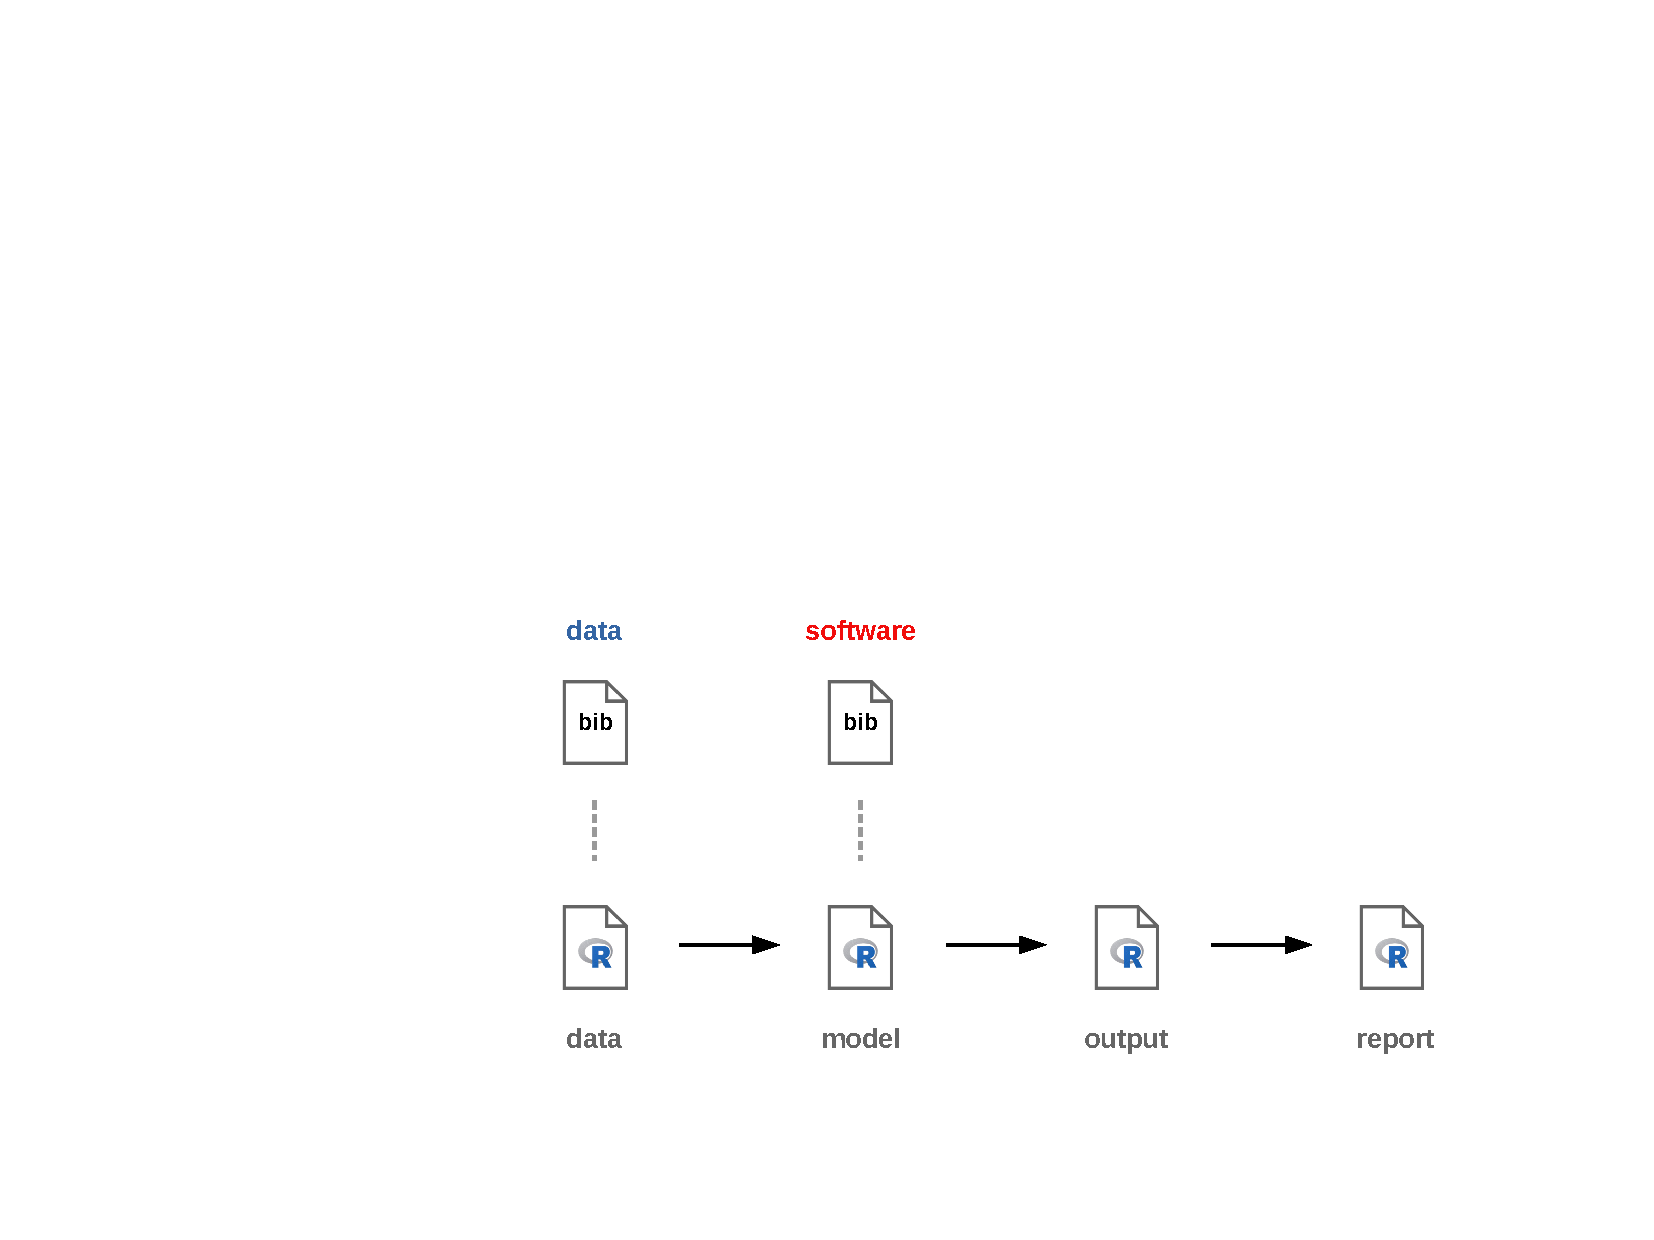
\includegraphics[width=0.7\textwidth]{diagram}
\end{frame}

% ______________________________________________________________________________

\begin{frame}{Design}\small
  \begin{itemize}
    \item[] The initial data that are used in the analysis are declared in a
    file called\\[0.2ex]
    {\bf\darkblue DATA.bib}, which is processed by the {\tt\blue taf.boot()}
    function.\\[4ex]
    During this boot procedure, each data entry is processed and the
    TAF\\[0.2ex]
    system then makes the data available in the {\tt boot/data}
    subfolder,\\[0.2ex]
    where the {\tt data.R} script will read it.\\[4ex]
    \item[] The {\bf\orange SOFTWARE.bib} file is optional. It is not used in
    the following\\
    linear regression example, but its functionality is covered in the slides\\
    on the boot procedure.
  \end{itemize}
\end{frame}

% ______________________________________________________________________________

\begin{frame}{Summary}
  \begin{itemize}
    \item[] {\bf\darkblue 1~ Background} \comment{objectives, design}\\[3ex]
    \item[] {\bf\darkblue 2~ Running a TAF analysis} \comment{linear regression,
      boot and run, structured scripts}\\[3ex]
    \item[] {\bf\darkblue 3~ TAF features} \comment{boot procedure, data flow,
      new analysis, overview of functions}\\[3ex]
    \item[] {\bf\darkblue 4~ The TAF community} \comment{browsing an existing
      analysis, related R packages}\\[3ex]
    \item[] {\bf\darkblue 5~ Discussion} \comment{contents of a TAF analysis,
      benefits of TAF}\\[3ex]
    \item[] {\bf\darkblue 6~ Online examples} \comment{ICES, FAO, SPC,
      various}\\[3ex]
  \end{itemize}
\end{frame}

\end{document}
